\documentclass{article}
\usepackage{graphicx} 

\title{Problem Set 8}
\author{Steven Plaisance}
\date{April 2023}

\begin{document}

\maketitle

\begin{enumerate}
  \item The closed-form solution provided very precise beta hat estimates, returning an average absolute error of .0017. This makes sense as the data provided was purely random.
  \item The gradient descent solution should work, though it did not return exceptional results for me. I believe this is because I only ran 1000 iterations, and I hope that more iterations would return better estimates. Gradient descent returned an average absolute error of 1.4.
  \item The L-BFGS algorithm returned very precise estimates, returning an average absolute error of .0017. These estimates were very marginally better than th estimates returned by the closed-form solution.
  \item The Nelder-Mead algorithm returned the most precise estimates, a rounded average absolute error of .00169, but marginally better than both the closed-form solution and the L-BFGS solution. 
  \item Finally, the linear regression returned an average absolute error of .0017, directly in line with both the closed-form solution and the L-BFGS. Please find the full linear regression results on the next page.
      \linebreak
    \linebreak
      \parbox{\linewidth}{
        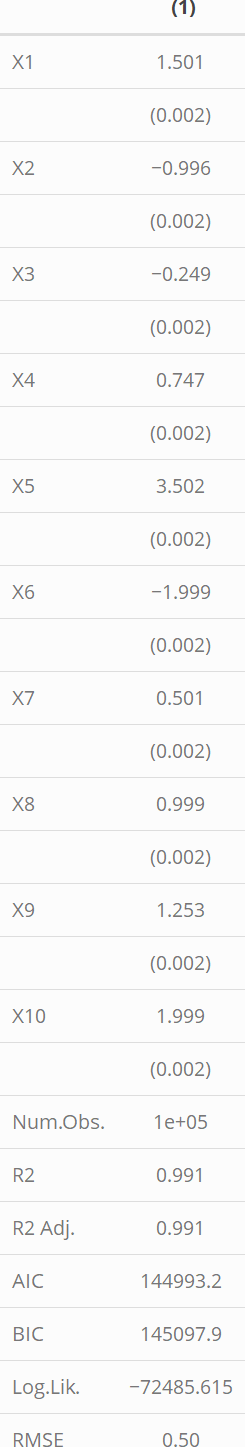
\includegraphics[width=3.5cm]{summaryTable.png}
        \centering
        \\}
\end{enumerate}
\end{document}
